\documentclass[10pt,a4paper,oneside]{article}

\usepackage[left=2.5cm,right=2.5cm,top=2.5cm,bottom=2.5cm]{geometry}

\usepackage[utf8]{inputenc}					% this is needed for german umlauts
%\usepackage[ngerman]{babel}					% this is needed for german umlauts
\usepackage[T1]{fontenc}						% this is needed for correct output 
                           					% of umlauts in pdf

\usepackage{lmodern}							% Latin Modern
\renewcommand*\familydefault{\sfdefault}		% Only if the base font of the document is to be sans serif
\usepackage[T1]{fontenc}

%%% Anfang: Anpassen des Layouts: Kopf- und Fußzeilen %%%

\usepackage{fancyhdr} 
\pagestyle{fancy} 
\fancyhf{} 									% alle Kopf- und Fußzeilenfelder bereinigen; 
											% löscht doppelte Seitenzahlen!
\fancyhead[L]{} 								% Kopfzeile links
\fancyhead[C]{}								% zentrierte Kopfzeile
\fancyhead[R]{} 								% Kopfzeile rechts
%\fancyhead[LO]{Test}						% Odd: ungerade Seiten
%\fancyhead[RO]{Test}
%\fancyhead[CO]{Test}
%\fancyhead[RE]{Test}						% Even: gerade Seiten
%\fancyhead[LE]{Test}
%\fancyhead[CE]{Test}
\fancyfoot[R]{\thepage} %Seitennummer

%\renewcommand{\headrulewidth}{0.4pt} %obere Trennlinie
%\renewcommand{\footrulewidth}{0.4pt} %untere Trennlinie

%%% Ende: Anpassen des Layouts: Kopf- und Fußzeilen %%%

\usepackage{graphicx}
\usepackage{xcolor}
\usepackage{wrapfig}

\definecolor{mygreen}{rgb}{0,0.6,0}
\definecolor{mygray}{rgb}{0.5,0.5,0.5}
\definecolor{mymauve}{rgb}{0.58,0,0.82}

\usepackage{color}							% Ermöglicht farbigen Text: \textcolor{declared-color}{text}
											% Bsp.: \textcolor{red}{Dieser Text ist rot}.
\usepackage{enumitem}

%%% Zeilenabstand %%%
\usepackage{setspace}
%\onehalfspacing %auskommentiert wird durchgehend einfacher Zeilenabstand verwendet

\newcommand{\qr}{\textquotedblleft}		% Definiert eine Abkürzung für dt. Anführungsstriche links
\newcommand{\ql}{\quotedblbase}			% Definiert eine Abkürzung für dt. Anführungsstriche rechts

\newcommand{\tabb}{\begin{tabbing}
m \= m \= m \= m \= m \= m \= m \= m \= m \= m \= m \kill}
\newcommand {\tabx}{\end{tabbing}}

\usepackage{booktabs}
\usepackage{tabularx}
\usepackage{listings}
\lstset{literate=
  {á}{{\'a}}1 {é}{{\'e}}1 {í}{{\'i}}1 {ó}{{\'o}}1 {ú}{{\'u}}1
  {Á}{{\'A}}1 {É}{{\'E}}1 {Í}{{\'I}}1 {Ó}{{\'O}}1 {Ú}{{\'U}}1
  {à}{{\`a}}1 {è}{{\`e}}1 {ì}{{\`i}}1 {ò}{{\`o}}1 {ù}{{\`u}}1
  {À}{{\`A}}1 {È}{{\'E}}1 {Ì}{{\`I}}1 {Ò}{{\`O}}1 {Ù}{{\`U}}1
  {ä}{{\"a}}1 {ë}{{\"e}}1 {ï}{{\"i}}1 {ö}{{\"o}}1 {ü}{{\"u}}1
  {Ä}{{\"A}}1 {Ë}{{\"E}}1 {Ï}{{\"I}}1 {Ö}{{\"O}}1 {Ü}{{\"U}}1
  {â}{{\^a}}1 {ê}{{\^e}}1 {î}{{\^i}}1 {ô}{{\^o}}1 {û}{{\^u}}1
  {Â}{{\^A}}1 {Ê}{{\^E}}1 {Î}{{\^I}}1 {Ô}{{\^O}}1 {Û}{{\^U}}1
  {œ}{{\oe}}1 {Œ}{{\OE}}1 {æ}{{\ae}}1 {Æ}{{\AE}}1 {ß}{{\ss}}1
  {ű}{{\H{u}}}1 {Ű}{{\H{U}}}1 {ő}{{\H{o}}}1 {Ő}{{\H{O}}}1
  {ç}{{\c c}}1 {Ç}{{\c C}}1 {ø}{{\o}}1 {å}{{\r a}}1 {Å}{{\r A}}1
  {€}{{\EUR}}1 {£}{{\pounds}}1
}
\lstset{ %
  backgroundcolor=\color{white},   % choose the background color; you must add \usepackage{color} or \usepackage{xcolor}
  basicstyle=\footnotesize,        % the size of the fonts that are used for the code
  breakatwhitespace=false,         % sets if automatic breaks should only happen at whitespace
  breaklines=true,                 % sets automatic line breaking
  captionpos=b,                    % sets the caption-position to bottom
  commentstyle=\color{mygreen},    % comment style
  deletekeywords={...},            % if you want to delete keywords from the given language
  escapeinside={\%*}{*)},          % if you want to add LaTeX within your code
  extendedchars=true,              % lets you use non-ASCII characters; for 8-bits encodings only, does not work with UTF-8
  frame=single,	                   % adds a frame around the code
  keepspaces=true,                 % keeps spaces in text, useful for keeping indentation of code (possibly needs columns=flexible)
  keywordstyle=\color{blue},       % keyword style
  language=Octave,                 % the language of the code
  otherkeywords={*,...},           % if you want to add more keywords to the set
  numbers=left,                    % where to put the line-numbers; possible values are (none, left, right)
  numbersep=5pt,                   % how far the line-numbers are from the code
  numberstyle=\tiny\color{mygray}, % the style that is used for the line-numbers
  rulecolor=\color{black},         % if not set, the frame-color may be changed on line-breaks within not-black text (e.g. comments (green here))
  showspaces=false,                % show spaces everywhere adding particular underscores; it overrides 'showstringspaces'
  showstringspaces=false,          % underline spaces within strings only
  showtabs=false,                  % show tabs within strings adding particular underscores
  stepnumber=1,                    % the step between two line-numbers. If it's 1, each line will be numbered
  stringstyle=\color{mymauve},     % string literal style
  tabsize=2,	                   % sets default tabsize to 2 spaces
  title=\lstname                   % show the filename of files included with \lstinputlisting; also try caption instead of title
}


%%% Nuetzliche Befehle:
%Behauptung \footnote{Beweis}; wird automatisch durchnummeriert 

%%% Anfang: Generelle Inforationen über das Dokument %%%

\author{Kilian Engelhardt}
\title{Technische Dokumentation}
\date{\today}

\usepackage{hyperref}					% Weitere Optionen unter:
										% http://de.wikibooks.org/wiki/LaTeX-W%C3%B6rterbuch:_hyperref
\hypersetup{								% Hier werden Informationen für das PDF gesetzt
pdftitle={},
pdfauthor={},
pdfsubject={},
pdfkeywords={},
colorlinks=true,							
linkcolor=black							% Definiert die Farbe der Links vom Inhaltsverzeichnis
}										% zu den Sections im Dokument

%%% Ende: Generelle Inforationen über das Dokument %%%

\setcounter{secnumdepth}{0} 				% Entfernt Nummerierung im TOC
\begin{document}
\pagestyle{empty}
\begin{titlepage}
	\begin{center}
		{\Large{\bf Technische Dokumentation}}
	\end{center}
\vspace{2cm}
	\begin{center}
		{\LARGE{\bf Umsetzung eines IPv6-Netzwerksegmentes mit Internetanbindung für die FastForward GmbH}}
	\end{center}
\vspace{1cm}
	\begin{center}
		Jahresprojekt der FS22 HHBK, 20. April 2016
	\end{center}
\vfill
	\begin{flushleft}
		Geplant und umgesetzt von:\newline
		Kilian Engelhardt \\
		Mirko Großmann \\
		Tom Vogler
	\end{flushleft}
\end{titlepage}

\tableofcontents
\newpage
\pagestyle{fancy}
\setcounter{page}{1}

\section{Anmerkungen}

Alle im Projekt verwendeten Passwörter wurden aus Datenschutzgründen in der Dokumentation durch die Zeichenfolge \ql password123\qr\ ersetzt. Alle Kommandoaufrufe wurden zur Vereinfachung als Benutzer root in einer Bash-Shell ausgeführt.\footnote{Um Verwechslungen in der Dokumentation durch ständiges Wechseln zwischen einem Normalbenutzer und dem Superuser, sowie die Verwendung von sudo-Aufrufen und unnötige Komplikationen mit Zugriffsrechten zu vermeiden.} Folgt einer Zeile mit einem Kommandoaufruf das Zeichen \textbackslash\ (Backslash), so gehört die nächste Zeile ebenfalls zum Kommandoaufruf.\footnote{Auszug aus man bash: \ql A non-quoted backslash (\textbackslash) is the escape character. It preserves the literal value of the next character that follows, with the exception of <newline>. If a <newline> pair appears, and the backslash is not itself quoted, the <newline> is treated as a line continuation (that is, it is removed from the input stream and effectively ignored).\qr}\newline

\noindent Darstellung von Kommandozeilenaufrufen:
\begin{lstlisting}[numbers=none]
> Kommandozeilenaufrufe werden in einem weißen Kasten in Monospace mit einem \
  vorangestellten > (Größer-als-Zeichen) dargestellt.
\end{lstlisting}
\noindent Darstellung von Konfigurationen:
\begin{lstlisting}
Konfigurationen werden ähnlich wie Kommandozeileaufrufe in einem weißen Kasten  
dargestellt, jedoch mit nummerierten Zeilen.
\end{lstlisting}

%\section{Informationen}

\subsection{Verwendete Hardware}

\begin{itemize}
	\item Router: Cisco 2801
	\item Switch: Cisco C2960
	\item no-name Server:
		\begin{itemize}
			\item[CPU] AMD Phenom X2 II 965 4x 3,4Ghz
			\item[RAM] 4x Kingston DDR3-1333Mhz 4GB
			\item[SSD] OCZ-VERTEX3 60GB
			\item[HDD] Hitachi HDS72105 500GB
			\item[LAN] 4x Gigabit-Ethernet
			\item Linux-Server
				\begin{itemize}
					\item[vCPUs] 1
					\item[RAM] 4GB
					\item[HDD] 100GB
				\end{itemize}
			\item Domain Controler
				\begin{itemize}
					\item[vCPUs] 3
					\item[RAM] 8GB
					\item[HDD] 300GB
				\end{itemize}
		\end{itemize}
\end{itemize}

\subsection{DNS}

Folgende DNS-Einstellungen wurden vorgenommen, um den Linux-Server aus dem Internet über die Domain {\texttt fastforward.hhbk.de} erreichbar zu machen.
\begin{lstlisting}[numbers=none]
fastforward.hhbk.de.		A		212.72.180.241
fastforward.hhbk.de.		AAAA 	2001:4dd0:fc0b:a::4
fastforward.hhbk.de.		MX		fastforward.hhbk.de
\end{lstlisting}

\subsection{SixXS}

\subsection{Adresskonzept}

\begin{tabular}{|l|l|l|}
\hline
					& LAN: VLAN 20					& DMZ: VLAN 10 \\
Router				& 2001:4dd0:fc0b:f4::1/128		& 2001:4dd0:fc0b:a::1/128 \\
Switch				& 2001:4dd0:fc0b:f4::2/128		& 2001:4dd0:fc0b:a::2/128 \\
Hypervisor			& 2001:4dd0:fc0b:f4::3/128		& 2001:4dd0:fc0b:a::3/128 \\	
Linux-Server											& 2001:4dd0:fc0b:a::4/128 \\
Domain Controler 	& 2001:4dd0:fc0b:f4::5/128		& \\
Client01				& 2001:4dd0:fc0b:f4::a/128		& \\
Client02				& 2001:4dd0:fc0b:f4::b/128		& \\
Client03				& 2001:4dd0:fc0b:f4::c/128		& \\
\hline
\end{tabular}

\subsection{Netzwerkplan}

\begin{wrapfigure}{c}{0.5\textwidth}
\includegraphics[scale=0.5]{8gruppe_dokumentation_pictures/02_JahresProjekt_Netzwerkplan.png}
\label{realisiertes_netzwerk}
\caption{Realisiertes Netzwerk}
\end{wrapfigure}
\section{Router: Konfiguration}

Abweichend von der einleitenden Anmerkung wurden folgende Befehle unter Ciscos iOS verwendet, um die Konfiguration des Routers vorzunehmen.

\begin{lstlisting}[numbers=none]
#Basics
r1#conf t
r1(config)#enable secret password123
r1(config)#enable password password123
r1(config)#ipv6 unicast-routing
r1(config)#ip name-server 8.8.8.8

#Vlan Deklaration
r1#vlan database 
r1(vlan)#vlan 10
r1(vlan)#vlan 20
r1(vlan)#apply
r1(vlan)#exit

#Subinterface vlan 10
r1(config)#interface FastEthernet0/1.10
r1(config-subif)#description subinterface vlan 10
r1(config-subif)#encapsulation dot1Q 10
r1(config-subif)#ipv6 address 2001:4dd0:fc0b:a::1/64
r1(config-subif)#no shutdown
r1(config-subif)#exit

#Subinterface vlan 20
r1(config)#interface FastEthernet0/1.20
r1(config-subif)#description subinterface vlan 20
r1(config-subif)#encapsulation dot1Q 20 native
r1(config-subif)#ipv6 address 2001:4dd0:fc0b:f4::1/64
r1(config-subif)#no shutdown
r1(config-subif)#exit

#Interface ins Schulnetz
r1(config)#interface fastethernet 0/0
r1(config-if)#ip address 212.72.180.241 255.255.255.224
r1(config-if)#ip default-gateway 212.72.180.225
r1(config-if)#no shutdown
r1(config-if)#exit

#SSH
r1(config)#ip domain-name fastforward.hhbk.de
r1(config)#crypto key generate rsa general-keys modulus 1024
r1(config)#username admin privilege 15 secret password123
r1(config)#line vty 0 4
r1(config-line)#transport input telnet ssh
r1(config-line)#login local
r1(config-line)#end

#Routing
r1(config)#ip route 0.0.0.0 0.0.0.0 fastethernet 0/0
r1(config)#ipv6 route 2001:4dd0:fc0b:a::/64 FastEthernet0/1.10
r1(config)#ipv6 route 2001:4dd0:fc0b:f4::/64 FastEthernet0/1.20

r1(config)#interface Tunnel61
r1(config-if)#description 6in4 tunnel to SixXS
r1(config-if)#no ip address
r1(config-if)#ip tcp adjust-mss 1420
r1(config-if)#ipv6 address 2001:4dd0:ff00:147f::2/64
r1(config-if)#ipv6 enable
r1(config-if)#tunnel source fastethernet 0/0
r1(config-if)#tunnel destination 78.35.24.124
r1(config-if)#tunnel mode ipv6ip
r1(config-if)#exit
r1(config)#ipv6 route ::/0 Tunnel61

#Tunnel Prüfen
r1#show ip interface tunnel61
r1#show ipv6 interface tunnel61
\end{lstlisting}

Konfiguration der Firewall:
\begin{lstlisting}[numbers=none]
#Firewalling
r1(config)#ipv6 access-list from_wan_in
r1(config-ipv6-acl)#permit icmp any any
r1(config-ipv6-acl)#permit tcp any any eq 22
r1(config-ipv6-acl)#permit tcp any any eq www reflect dmz-wan-reflexive timeout 5
r1(config-ipv6-acl)#permit tcp any any eq 443 reflect dmz-wan-reflexive timeout 5
r1(config-ipv6-acl)#permit tcp any any eq smtp
r1(config-ipv6-acl)#evaluate wan-dmz-reflexive
r1(config-ipv6-acl)#evaluate wan-lan-reflexive

r1(config)#interface Tunnel61
r1(config-if)#ipv6 traffic-filter from_wan_in in

r1(config)#ipv6 access-list dmz_in
r1(config-ipv6-acl)#permit icmp any any
r1(config-ipv6-acl)#permit udp any any eq domain reflect wan-dmz-reflexive timeout 5
r1(config-ipv6-acl)#permit tcp any any eq 22 reflect wan-dmz-reflexive timeout 5
r1(config-ipv6-acl)#permit tcp any any eq www reflect wan-dmz-reflexive timeout 5
r1(config-ipv6-acl)#permit tcp any any eq 443 reflect wan-dmz-reflexive timeout 5
r1(config-ipv6-acl)#permit tcp any any eq smtp reflect wan-dmz-reflexive timeout 5
r1(config-ipv6-acl)#evaluate dmz-wan-reflexive

r1(config)#interface FastEthernet0/1.10
r1(config-if)#ipv6 traffic-filter dmz_in in

r1(config)#ipv6 access-list lan_in
r1(config-ipv6-acl)#permit icmp any any
r1(config-ipv6-acl)#permit udp any any eq domain reflect wan-lan-reflexive timeout 5
r1(config-ipv6-acl)#permit tcp any any eq 22 reflect wan-lan-reflexive timeout 5
r1(config-ipv6-acl)#permit tcp any any eq www reflect wan-lan-reflexive timeout 5
r1(config-ipv6-acl)#permit tcp any any eq 443 reflect wan-lan-reflexive timeout 5
r1(config-ipv6-acl)#permit tcp any any eq smtp reflect wan-lan-reflexive timeout 5
r1(config-ipv6-acl)#permit tcp any any eq ftp reflect wan-lan-reflexive timeout 5
r1(config-ipv6-acl)#permit tcp any any eq ftp-data reflect wan-lan-reflexive timeout 5

r1(config)#interface FastEthernet0/1.20
r1(config-if)#ipv6 traffic-filter lan_in in

r1(config)#interface FastEthernet0/0
r1(config-if)#ip access-group from_wan_in in

r1(config)#do show ipv6 access-list
\end{lstlisting}\section{Switch: Konfiguration}

Abweichend von der einleitenden Anmerkung wurden folgende Befehle unter Ciscos iOS verwendet, um die Konfiguration des Switches vorzunehmen.

\begin{lstlisting}[numbers=none]
#Basic
switch(config)#enable secret Willkommen2016
switch(config)#enable password Willkommen2016
switch(config)#sdm prefer dual-ipv4-and-ipv6
switch(config)#end
switch# reload

#Vlan Deklaration
switch#vlan database 
switch(vlan)#vlan 10
switch(vlan)#vlan 20
switch(vlan)#exit

#interface vlan 10
switch(config)#interface range gigabitEthernet f0/1-24 
Switch(config-if-range)#switchport access vlan 10
Switch(config-if-range)#end
Switch(config)#interface vlan 10
Switch(config-if)#ipv6 address 2001:4dd0:fc0b:a::2/64
Switch(config-if)#no shut down
Switch(config-if)#exit

#interface vlan 20
switch(config)# interface range gigabitEthernet f0/25-46
Switch(config-if-range)# switchport access vlan 20
Switch(config-if-range)# end
Switch(config)#interface vlan 20
Switch(config-if)#ipv6 address 2001:4dd0:fc0b:f4::2/64
Switch(config-if)#no shut down
Switch(config-if)# exit

#trunk
switch(config)#interface gigabitEthernet 0/43
Switch(config-if)#switchport mode trunk
Switch(config-if)#switchport trunk native vlan 20
Switch(config-if)#switchport trunk allowed vlan 10,20

#SSH
Switch(config)#ip domain-name fastforward.hhbk.de
Switch(config)#crypto key generate rsa general-keys modulus 1024
Switch(config)#username admin privilege 15 secret Willkommen2016
Switch(config)#line vty 0 4
Switch(config-line)#transport input telnet ssh
Switch(config-line)#login local
Switch(config-line)#en
\end{lstlisting}\section{Hypervisor}

\subsection{Installation}

Die Installation erfolgt per graphischen Installationsdialog. Englisch wurde gewählt, da es die Lingua franca in der IT darstellt. Zusätzlich wurde OpenSSH bei der Installation ausgewählt, um den Server ohne graphische Oberfläche aus der Ferne zu administrieren. Insgesamt wurden während der Installation folgende Einstellungen vorgenommen:
\begin{itemize}
	\item[Language] Englisch
	\item[Territory] Germany
	\item[Keyboard] german
	\item[Hostname] hypervisor
	\item[Domain name] fastforward.hhbk.de
	\item[Username] user
	\item[Password] password123
	\item[Paritioning] Guided: use entire disk
	\item[Choose software] Default, OpenSSH
	\item[Grub MBR] sdb
\end{itemize}

Nach der Installation wurde darüberhinaus folgende Software installiert: {\sc qemu-kvm libvirt-bin virtinst}.

\subsection{Konfiguration}

\subsubsection{libvirt}

Zunächst muss der QEMU-Treiber von {\sc libvirt} konfiguriert werden, damit dieser weiß, mit welchem User QEMU ausgeführt wird. 

Konfigurationsdatei: {\sc /etc/libvirt/qemu.conf}
\begin{lstlisting}
user = "root"
group = "root"
\end{lstlisting}

Anschließend wird die HDD mit 500GB formatiert und die Volume Group {\sc vg0} definiert.

\begin{lstlisting}[numbers=none]
> parted /dev/sda
   mklabel GPT
   mkpart primary 1M 100%
   set 1 lvm on
> pvcreate /dev/sda1
> vgcreate vg0 /dev/sda1
\end{lstlisting} 

Die Volume Group {\sc vg0} wird verwendet, um den Pool {\sc vg0} einzurichten. Die folgende Konfiguration muss erstellt werden, um anschließend mit den aufgeführten Befehlen den Pool zu aktivieren.       

Konfigurationsdatei: {\sc /etc/libvirt/qemu/storage/vg0.xml}
\begin{lstlisting}
<pool type='logical'>
        <name>vg0</name>
        <source>
                <device path='/dev/sda1'/>
        </source>
        <target>
                <path>/dev/vg0</path>
        </target>
</pool>
\end{lstlisting}
\begin{lstlisting}[numbers=none]
> virsh pool-define /etc/libvirt/qemu/storage/vg0.xml
> virsh pool-start vg0
> virsh pool-autostart vg0
\end{lstlisting}

\subsubsection{Netzwerk}

Der Hypervisor wurde mit zwei Interfaces an den Switch angebunden. Das Interface {\sc enp4s0} wurde an einen Port mit VLAN 10 angeschlossen und {\sc enp2s0} an einen Port mit VLAN 20. Dadurch ist es später einfacher, die virtuellen Server einem VLAN zuzuordnen (s. Kapitel \ql Linux-Server\qr). Für DNS wurde ein Server von Google ausgewählt.

Konfigurationsdatei: {\sc /etc/network/interfaces}
\begin{lstlisting}
source /etc/network/interfaces.d/*

# The loopback network interface
auto lo
iface lo inet loopback

# The primary network interface
auto enp4s0
iface enp4s0 inet manual
        dns-nameservers 2001:4860:4860::8888

auto enp2s0
iface enp2s0 inet manual
        dns-nameservers 2001:4860:4860::8888

auto br0
iface br0 inet manual

iface br0 inet6 static
        bridge_ports    enp4s0
        address 2001:4dd0:fc0b:a::3
        netmask 64
        gateway 2001:4dd0:fc0b:a::1

auto br1
iface br1 inet manual

iface br1 inet6 static
        bridge_ports    enp2s0
        address 2001:4dd0:fc0b:f4::3
        netmask 64
\end{lstlisting}\section{Linux-Server}

\subsection{Installation}

Die virtuelle Maschine wurde auf dem Hypervisor mithilfe von {\sc virtinst} und folgendem Befehl initialisiert.

\begin{lstlisting}[numbers=none]
> virt-install --connect qemu:///system --hvm --name webserver --ram 4096 --vcpus 1 \
  --disk pool=vg0,size=100,bus=virtio,cache=none,sparse=false \
  --cdrom=/root/isos/ubuntu-16.04-server-amd64.iso --os-type linux \
  --network bridge=br0,model=virtio \
  --graphics vnc,port=10123,listen=0.0.0.0,keymap=de,password=password123 \
  --boot cdrom
\end{lstlisting}

Über die IP des Hypervisors und den Port $10123$ wurde eine Verbindung per VNC hergestellt, um anschließend die Installation per graphischem Installationsdialog durchzuführen. Englisch wurde gewählt, da es die Lingua franca in der IT darstellt. Zusätzlich wurde OpenSSH bei der Installation ausgewählt, um den Server ohne graphische Oberfläche aus der Ferne zu administrieren. Insgesamt wurden während der Installation folgende Einstellungen vorgenommen:
\begin{itemize}
	\item[Language] Englisch
	\item[Territory] Germany
	\item[Keyboard] german
	\item[Hostname] webserver
	\item[Domain name] fastforward.hhbk.de
	\item[Username] user
	\item[Password] password123
	\item[Paritioning] Guided: use entire disk
	\item[Choose software] Default, OpenSSH
	\item[Grub MBR] vda
\end{itemize}

Nach der Installation wurde darüberhinaus folgende Software installiert: {\sc apache2 postfix}.

\subsection{Konfiguration}

Nach der Installation von Apache wurde die Defaultwebseite durch eine ersetzt, die \ql Hello World!\qr\ ausliefert.

Konfigurationsdatei: {\sc /var/www/html/index.html}
\begin{lstlisting}
Hello World!
\end{lstlisting}

Während des Installationsdialoges von Postfix wurde \ql Internet with Smarthost\qr\ gewählt. Der SMTP-Server bleibt unkonfiguriert. Als Domain wird \ql fastforward.hhbk.de\qr\ angegeben.

\subsubsection{Netzwerk}

Konfigurationsdatei: {\sc /etc/network/interfaces}
\begin{lstlisting}
source /etc/network/interfaces.d/*

# The loopback network interface
auto lo
iface lo inet loopback

# The primary network interface
auto ens3
iface ens3 inet manual

iface ens3 inet6 static
        address			2001:4dd0:fc0b:a::4
        netmask			64
        gateway			2001:4dd0:fc0b:a::1
        dns-nameservers	2001:4860:4860::8888
\end{lstlisting}

\section{Domain Controler}

\subsection{Installation}

Die virtuelle Maschine wurde auf dem Hypervisor mithilfe von {\sc virtinst} und folgendem Befehl initialisiert.

\begin{lstlisting}[numbers=none]
> virt-install --hvm --connect qemu:///system --name win2012 --ram 8192 --vcpus 2 \
  --disk pool=vg0,size=300,bus=virtio,cache=none,sparse=false \
  --disk path=/root/isos/virtio-win.iso,device=cdrom,perms=ro \
  --cdrom /root/isos/win2012r2.iso \
  --os-type windows \
  --network bridge=br0,model=virtio \
  --graphics vnc,port=10234,listen=0.0.0.0,keymap=de,password=password123 \
  --boot cdrom,hd,menu=on
\end{lstlisting}

Anschließend wurde sich per VNC verbunden, um den Domain Controler per graphischem Installationsdialog zu installieren. Dabei wurde eine Installation mit graphischer Oberfläche gewählt, da dies der üblichen Administrationsweise unter Windows entspricht. Während der Installation müssen über die zusätzlich eingebundene CD \ql virtio-win\qr\ die Treiber für das Netzwerk ({\sc NetKVM > WIN2012R2 > amd64}) und die Festplatte ({\sc viostor > WIN2012	R2 > amd64})installiert werden. Bei der Partitionierung wurde die gesamte Festplatte gewählt und abschließend dem Administrator das Passwort \ql password123\qr\ gegeben.

\subsection{Konfiguration}\section{Windows Client}

\subsection{Installation}
\subsection{Konfiguration}\section{Tests}

\subsection{Erreichbarkeit intern}

Mit dem folgenen Skript wurde die allgemeine Erreichbarkeit der Server aus dem LAN getestet.

Shell-Skript: {\sc test-ping.sh}
\begin{lstlisting}
#!/bin/bash

#killall dhclient

RIP1="2001:4dd0:fc0b:a::1"
RIP2="2001:4dd0:fc0b:f4::1"
SIP1="2001:4dd0:fc0b:a::2"
SIP2="2001:4dd0:fc0b:f4::2"
KVM1="2001:4dd0:fc0b:a::3"
KVM2="2001:4dd0:fc0b:f4::3"
SRV="2001:4dd0:fc0b:a::4"
DC="2001:4dd0:fc0b:f4::5"

LOG="test-ping_$(date +%Y%d%m).log"

IP="${RIP1} ${RIP2} ${SIP1} ${SIP2} ${KVM1} ${KVM2} ${SRV} ${DC}"

echo -e "##########" >> ${LOG}
echo -e "Ping-Test $(date +%Y%m%d):\n" >> ${LOG}
for i in ${IP}; do
	ping6 -c 1 ${i} 2> /dev/null
	if [[ $? -eq 0 ]]; then
		echo -e "${i}\t\tworks" >> ${LOG}
	else
		echo -e "${i}\t\tfailed!" >> ${LOG}
	fi
done	
echo -e "\n" >> ${LOG}
\end{lstlisting}

Log-Datei: {\sc test-ping_20160622.log}
\begin{lstlisting}
##########
Ping-Test 20160622:

2001:4dd0:fc0b:a::1		works
2001:4dd0:fc0b:f4::1		works
2001:4dd0:fc0b:a::2		works
2001:4dd0:fc0b:f4::2		works
2001:4dd0:fc0b:a::3		works
2001:4dd0:fc0b:f4::3		works
2001:4dd0:fc0b:a::4		works
2001:4dd0:fc0b:f4::5		works
\end{lstlisting}

\subsection{Erreichbarkeit extern}

\subsubsection{Allgemeine Erreichbarkeit}

Zum Testen der allgemeinen Erreichbarkeit von extern wurde der Ping-Test an einem Internetanschluss mit Dualstack wiederholt.

\begin{lstlisting}
##########
Ping-Test 20160622:

2001:4dd0:fc0b:a::1		works
2001:4dd0:fc0b:f4::1		works
2001:4dd0:fc0b:a::2		works
2001:4dd0:fc0b:f4::2		works
2001:4dd0:fc0b:a::3		works
2001:4dd0:fc0b:f4::3		works
2001:4dd0:fc0b:a::4		works
2001:4dd0:fc0b:f4::5		works
\end{lstlisting}

\subsubsection{Erreichbarkeit Webserver}

Die Erreichbarkeit des Webservers wurde von der Kommandozeile per {\sc curl} getestet.

\begin{lstlisting}[numbers=none]
> curl -v fastforward.hhbk.de
 * Rebuilt URL to: fastforward.hhbk.de/
 * Hostname was NOT found in DNS cache
 *   Trying 2001:4dd0:fc0b:a::4...
 * Connected to fastforward.hhbk.de (2001:4dd0:fc0b:a::4) port 80 (#0)
 > GET / HTTP/1.1
 > User-Agent: curl/7.35.0
 > Host: fastforward.hhbk.de
 > Accept: */*
 > 
 < HTTP/1.1 200 OK
 < Date: Wed, 22 Jun 2016 15:03:00 GMT
 * Server Apache/2.4.18 (Ubuntu) is not blacklisted
 < Server: Apache/2.4.18 (Ubuntu)
 < Last-Modified: Mon, 20 Jun 2016 07:40:59 GMT
 < ETag: "d-535b0d3581c7e"
 < Accept-Ranges: bytes
 < Content-Length: 13
 < Content-Type: text/html
 < 
 Hello World!
 * Connection #0 to host fastforward.hhbk.de left intact
\end{lstlisting}

\subsubsection{Erreichbarkeit Mailserver}

Die Erreichbarkeit des Mailservers wurde von der Kommandozeile per {\sc telnet} getestet.

\begin{lstlisting}[numbers=none]
> telnet fastforward.hhbk.de 25
 Trying 2001:4dd0:fc0b:a::4...
 Connected to fastforward.hhbk.de.
 Escape character is '^]'.
 220 webserver ESMTP Postfix (Ubuntu)
 HELO fastforward.hhbk.de
 250 webserver
 mail from: <test@test.com>
 250 2.1.0 Ok
 rcpt to: <kilian@fastforward.hhbk.de>
 250 2.1.5 Ok
 subject: test
 Line one
 Line two
 .
 250 2.0.0 Ok: queued as 1BF1B6099B
 quit
 221 2.0.0 Bye
 Connection closed by foreign host.
\end{lstlisting}

\begin{lstlisting}[numbers=none]
> tail /var/mail/kilian 
 X-Original-To: kilian@fastforward.hhbk.de
 Delivered-To: kilian@fastforward.hhbk.de
 Received: from fastforward.hhbk.de (unknown [IPv6:2a02:908:1251:7160:495e:958d:9e35:f017])
	by webserver (Postfix) with SMTP id 1BF1B6099B
	for <kilian@fastforward.hhbk.de>; Wed, 22 Jun 2016 16:49:47 +0200 (CEST)

 subject: test
 Line one
 Line two
\end{lstlisting}

\subsection{Firewall}

Mit den folgenden Kommandos wurde getestet, ob die Firewall nicht freigeschaltete Ports blockiert. Dazu wurde auf dem Linux-Server mit {\sc netcat} ein Port geöffnet und von extern geprüft, ob sich zu diesem Port verbunden werden kann.

\begin{lstlisting}
 #Listening auf dem Linux-Server
> netcat -l -p 1337

 #Vom externen Host
> telnet 2001:4dd0:fc0b:a::4 1337
 Trying 2001:4dd0:fc0b:a::4...
 telnet: connect to address 2001:4dd0:fc0b:a::4: Permission denied
\end{lstlisting}

\section{Informationen}

\subsection{Verwendete Hardware}

\begin{itemize}
	\item Router: Cisco 2801
	\item Switch: Cisco C2960
	\item no-name Server:
		\begin{itemize}
			\item[CPU] AMD Phenom X2 II 965 4x 3,4Ghz
			\item[RAM] 4x Kingston DDR3-1333Mhz 4GB
			\item[SSD] OCZ-VERTEX3 60GB
			\item[HDD] Hitachi HDS72105 500GB
			\item[LAN] 4x Gigabit-Ethernet
			\item Linux-Server
				\begin{itemize}
					\item[vCPUs] 1
					\item[RAM] 4GB
					\item[HDD] 100GB
				\end{itemize}
			\item Domain Controler
				\begin{itemize}
					\item[vCPUs] 3
					\item[RAM] 8GB
					\item[HDD] 300GB
				\end{itemize}
		\end{itemize}
\end{itemize}

\subsection{DNS}

Folgende DNS-Einstellungen wurden vorgenommen, um den Linux-Server aus dem Internet über die Domain {\texttt fastforward.hhbk.de} erreichbar zu machen.
\begin{lstlisting}[numbers=none]
fastforward.hhbk.de.		A			212.72.180.241
fastforward.hhbk.de.		AAAA 	2001:4dd0:fc0b:a::4
fastforward.hhbk.de.		MX		fastforward.hhbk.de
\end{lstlisting}

\subsection{SixXS}

Folgende Daten wurden verwendet, um mit einem CISCO Router einen IPv6 via IPv4 Tunnel mit SixXS auf zu bauen.


\begin{tabular}{|l|l|}
\hline
Beschreibung			& Daten						\\
\hline
Router IP				& 212.72.180.241		 	\\
SixXS PoP IPv4			& 78.35.24.124			 	\\
IPv6 Prefix				& /64					 	\\	
Lokaler Router	IPv6	& 2001:4dd0:ff00:147f::2 	\\
SixXS Router IPv6 		& 2001:4dd0:ff00:147f::1	\\
TCP Adjust-MSS			& 1420						\\
Tunnel Mode				& ipv6ip					\\
\hline
\end{tabular}

\subsection{Adresskonzept}

\begin{tabular}{|l|l|l|}
\hline
						& LAN: VLAN 20					& DMZ: VLAN 10 \\
\hline
Router					& 2001:4dd0:fc0b:f4::1/128		& 2001:4dd0:fc0b:a::1/128 \\
Switch					& 2001:4dd0:fc0b:f4::2/128		& 2001:4dd0:fc0b:a::2/128 \\
Hypervisor				& 2001:4dd0:fc0b:f4::3/128		& 2001:4dd0:fc0b:a::3/128 \\	
Linux-Server			&								& 2001:4dd0:fc0b:a::4/128 \\
Domain Controler 		& 2001:4dd0:fc0b:f4::5/128		& \\
Client01				& 2001:4dd0:fc0b:f4::a/128		& \\
Client02				& 2001:4dd0:fc0b:f4::b/128		& \\
Client03				& 2001:4dd0:fc0b:f4::c/128		& \\
\hline
\end{tabular}

\subsection{Netzwerkplan}

%\begin{wrapfigure}{c}{0.5\textwidth}
\includegraphics[scale=0.5]{8gruppe_dokumentation_pictures/02_JahresProjekt_Netzwerkplan.png}
\label{realisiertes_netzwerk}
%\caption{Realisiertes Netzwerk}
%\end{wrapfigure}

\section{Router: Konfiguration}

Abweichend von der einleitenden Anmerkung wurden folgende Befehle unter Ciscos iOS verwendet, um die Konfiguration des Routers vorzunehmen.

\begin{lstlisting}[numbers=none]
#Basics
r1#conf t
r1(config)#enable secret password123
r1(config)#enable password password123
r1(config)#ipv6 unicast-routing
r1(config)#ip name-server 8.8.8.8

#Vlan Deklaration
r1#vlan database 
r1(vlan)#vlan 10
r1(vlan)#vlan 20
r1(vlan)#apply
r1(vlan)#exit

#Subinterface vlan 10
r1(config)#interface FastEthernet0/1.10
r1(config-subif)#description subinterface vlan 10
r1(config-subif)#encapsulation dot1Q 10
r1(config-subif)#ipv6 address 2001:4dd0:fc0b:a::1/64
r1(config-subif)#no shutdown
r1(config-subif)#exit

#Subinterface vlan 20
r1(config)#interface FastEthernet0/1.20
r1(config-subif)#description subinterface vlan 20
r1(config-subif)#encapsulation dot1Q 20 native
r1(config-subif)#ipv6 address 2001:4dd0:fc0b:f4::1/64
r1(config-subif)#no shutdown
r1(config-subif)#exit

#Interface ins Schulnetz
r1(config)#interface fastethernet 0/0
r1(config-if)#ip address 212.72.180.241 255.255.255.224
r1(config-if)#ip default-gateway 212.72.180.225
r1(config-if)#no shutdown
r1(config-if)#exit

#SSH
r1(config)#ip domain-name fastforward.hhbk.de
r1(config)#crypto key generate rsa general-keys modulus 1024
r1(config)#username admin privilege 15 secret password123
r1(config)#line vty 0 4
r1(config-line)#transport input telnet ssh
r1(config-line)#login local
r1(config-line)#end

#Routing
r1(config)#ip route 0.0.0.0 0.0.0.0 fastethernet 0/0
r1(config)#ipv6 route 2001:4dd0:fc0b:a::/64 FastEthernet0/1.10
r1(config)#ipv6 route 2001:4dd0:fc0b:f4::/64 FastEthernet0/1.20

r1(config)#interface Tunnel61
r1(config-if)#description 6in4 tunnel to SixXS
r1(config-if)#no ip address
r1(config-if)#ip tcp adjust-mss 1420
r1(config-if)#ipv6 address 2001:4dd0:ff00:147f::2/64
r1(config-if)#ipv6 enable
r1(config-if)#tunnel source fastethernet 0/0
r1(config-if)#tunnel destination 78.35.24.124
r1(config-if)#tunnel mode ipv6ip
r1(config-if)#exit
r1(config)#ipv6 route ::/0 Tunnel61

#Tunnel Prüfen
r1#show ip interface tunnel61
r1#show ipv6 interface tunnel61
\end{lstlisting}

Konfiguration der Firewall:
\begin{lstlisting}[numbers=none]
#Firewalling
r1(config)#ipv6 access-list from_wan_in
r1(config-ipv6-acl)#permit icmp any any
r1(config-ipv6-acl)#permit tcp any any eq 22
r1(config-ipv6-acl)#permit tcp any any eq www reflect dmz-wan-reflexive timeout 5
r1(config-ipv6-acl)#permit tcp any any eq 443 reflect dmz-wan-reflexive timeout 5
r1(config-ipv6-acl)#permit tcp any any eq smtp
r1(config-ipv6-acl)#evaluate wan-dmz-reflexive
r1(config-ipv6-acl)#evaluate wan-lan-reflexive

r1(config)#interface Tunnel61
r1(config-if)#ipv6 traffic-filter from_wan_in in

r1(config)#ipv6 access-list dmz_in
r1(config-ipv6-acl)#permit icmp any any
r1(config-ipv6-acl)#permit udp any any eq domain reflect wan-dmz-reflexive timeout 5
r1(config-ipv6-acl)#permit tcp any any eq 22 reflect wan-dmz-reflexive timeout 5
r1(config-ipv6-acl)#permit tcp any any eq www reflect wan-dmz-reflexive timeout 5
r1(config-ipv6-acl)#permit tcp any any eq 443 reflect wan-dmz-reflexive timeout 5
r1(config-ipv6-acl)#permit tcp any any eq smtp reflect wan-dmz-reflexive timeout 5
r1(config-ipv6-acl)#evaluate dmz-wan-reflexive

r1(config)#interface FastEthernet0/1.10
r1(config-if)#ipv6 traffic-filter dmz_in in

r1(config)#ipv6 access-list lan_in
r1(config-ipv6-acl)#permit icmp any any
r1(config-ipv6-acl)#permit udp any any eq domain reflect wan-lan-reflexive timeout 5
r1(config-ipv6-acl)#permit tcp any any eq 22 reflect wan-lan-reflexive timeout 5
r1(config-ipv6-acl)#permit tcp any any eq www reflect wan-lan-reflexive timeout 5
r1(config-ipv6-acl)#permit tcp any any eq 443 reflect wan-lan-reflexive timeout 5
r1(config-ipv6-acl)#permit tcp any any eq smtp reflect wan-lan-reflexive timeout 5
r1(config-ipv6-acl)#permit tcp any any eq ftp reflect wan-lan-reflexive timeout 5
r1(config-ipv6-acl)#permit tcp any any eq ftp-data reflect wan-lan-reflexive timeout 5

r1(config)#interface FastEthernet0/1.20
r1(config-if)#ipv6 traffic-filter lan_in in

r1(config)#interface FastEthernet0/0
r1(config-if)#ip access-group from_wan_in in

r1(config)#do show ipv6 access-list
\end{lstlisting}
\section{Switch: Konfiguration}

Abweichend von der einleitenden Anmerkung wurden folgende Befehle unter Ciscos iOS verwendet, um die Konfiguration des Switches vorzunehmen.

\begin{lstlisting}[numbers=none]
#Basic
switch(config)#enable secret Willkommen2016
switch(config)#enable password Willkommen2016
switch(config)#sdm prefer dual-ipv4-and-ipv6
switch(config)#end
switch# reload

#Vlan Deklaration
switch#vlan database 
switch(vlan)#vlan 10
switch(vlan)#vlan 20
switch(vlan)#exit

#interface vlan 10
switch(config)#interface range gigabitEthernet f0/1-24 
Switch(config-if-range)#switchport access vlan 10
Switch(config-if-range)#end
Switch(config)#interface vlan 10
Switch(config-if)#ipv6 address 2001:4dd0:fc0b:a::2/64
Switch(config-if)#no shut down
Switch(config-if)#exit

#interface vlan 20
switch(config)# interface range gigabitEthernet f0/25-46
Switch(config-if-range)# switchport access vlan 20
Switch(config-if-range)# end
Switch(config)#interface vlan 20
Switch(config-if)#ipv6 address 2001:4dd0:fc0b:f4::2/64
Switch(config-if)#no shut down
Switch(config-if)# exit

#trunk
switch(config)#interface gigabitEthernet 0/43
Switch(config-if)#switchport mode trunk
Switch(config-if)#switchport trunk native vlan 20
Switch(config-if)#switchport trunk allowed vlan 10,20

#SSH
Switch(config)#ip domain-name fastforward.hhbk.de
Switch(config)#crypto key generate rsa general-keys modulus 1024
Switch(config)#username admin privilege 15 secret Willkommen2016
Switch(config)#line vty 0 4
Switch(config-line)#transport input telnet ssh
Switch(config-line)#login local
Switch(config-line)#en
\end{lstlisting}
\section{Hypervisor}

\subsection{Installation}

Die Installation erfolgt per graphischen Installationsdialog. Englisch wurde gewählt, da es die Lingua franca in der IT darstellt. Zusätzlich wurde OpenSSH bei der Installation ausgewählt, um den Server ohne graphische Oberfläche aus der Ferne zu administrieren. Insgesamt wurden während der Installation folgende Einstellungen vorgenommen:
\begin{itemize}[leftmargin=+1in]
	\item[Language] Englisch
	\item[Territory] Germany
	\item[Keyboard] german
	\item[Hostname] hypervisor
	\item[Domain name] fastforward.hhbk.de
	\item[Username] user
	\item[Password] password123
	\item[Paritioning] Guided: use entire disk
	\item[Choose software] Default, OpenSSH
	\item[Grub MBR] sdb
\end{itemize}

Nach der Installation wurde darüberhinaus folgende Software installiert: {\texttt qemu-kvm libvirt-bin virtinst}.

\subsection{Konfiguration}

\subsubsection{libvirt}

Zunächst muss der QEMU-Treiber von {\texttt libvirt} konfiguriert werden, damit dieser weiß, mit welchem User QEMU ausgeführt wird.\newline

Konfigurationsdatei: {\texttt /etc/libvirt/qemu.conf}
\begin{lstlisting}
user = "root"
group = "root"
\end{lstlisting}

Anschließend wird die HDD mit 500GB formatiert und die Volume Group {\texttt vg0} definiert.\newline

\begin{lstlisting}[numbers=none]
> parted /dev/sda
   mklabel GPT
   mkpart primary 1M 100%
   set 1 lvm on
> pvcreate /dev/sda1
> vgcreate vg0 /dev/sda1
\end{lstlisting} 

Die Volume Group {\texttt vg0} wird verwendet, um den Pool {\texttt vg0} einzurichten. Die folgende Konfiguration muss erstellt werden, um anschließend mit den aufgeführten Befehlen den Pool zu aktivieren.

\newpage
Konfigurationsdatei: {\texttt /etc/libvirt/qemu/storage/vg0.xml}
\begin{lstlisting}
<pool type='logical'>
        <name>vg0</name>
        <source>
                <device path='/dev/sda1'/>
        </source>
        <target>
                <path>/dev/vg0</path>
        </target>
</pool>
\end{lstlisting}
\begin{lstlisting}[numbers=none]
> virsh pool-define /etc/libvirt/qemu/storage/vg0.xml
> virsh pool-start vg0
> virsh pool-autostart vg0
\end{lstlisting}

\subsubsection{Netzwerk}

Der Hypervisor wurde mit zwei Interfaces an den Switch angebunden. Das Interface {\texttt enp4s0} wurde an einen Port mit VLAN 10 angeschlossen und {\texttt enp2s0} an einen Port mit VLAN 20. Dadurch ist es später einfacher, die virtuellen Server einem VLAN zuzuordnen (s. Kapitel \ql Linux-Server\qr). Für DNS wurde ein Server von Google ausgewählt.\newline

Konfigurationsdatei: {\texttt /etc/network/interfaces}
\begin{lstlisting}
source /etc/network/interfaces.d/*

# The loopback network interface
auto lo
iface lo inet loopback

# The primary network interface
auto enp4s0
iface enp4s0 inet manual
        dns-nameservers 2001:4860:4860::8888

auto enp2s0
iface enp2s0 inet manual
        dns-nameservers 2001:4860:4860::8888

auto br0
iface br0 inet manual

iface br0 inet6 static
        bridge_ports    enp4s0
        address 2001:4dd0:fc0b:a::3
        netmask 64
        gateway 2001:4dd0:fc0b:a::1

auto br1
iface br1 inet manual

iface br1 inet6 static
        bridge_ports    enp2s0
        address 2001:4dd0:fc0b:f4::3
        netmask 64
\end{lstlisting}

\section{Domain Controler: Installation und Konfiguration}
\section{Domain Controler}

\subsection{Installation}

Die virtuelle Maschine wurde auf dem Hypervisor mithilfe von {\texttt virtinst} und folgendem Befehl initialisiert.

\begin{lstlisting}[numbers=none]
> virt-install --hvm --connect qemu:///system --name win2012 --ram 8192 --vcpus 2 \
  --disk pool=vg0,size=300,bus=virtio,cache=none,sparse=false \
  --disk path=/root/isos/virtio-win.iso,device=cdrom,perms=ro \
  --cdrom /root/isos/win2012r2.iso \
  --os-type windows \
  --network bridge=br0,model=virtio \
  --graphics vnc,port=10234,listen=0.0.0.0,keymap=de,password=password123 \
  --boot cdrom,hd,menu=on
\end{lstlisting}

Anschließend wurde sich per VNC verbunden, um den Domain Controler per graphischem Installationsdialog zu installieren. Dabei wurde eine Installation mit graphischer Oberfläche gewählt, da dies der üblichen Administrationsweise unter Windows entspricht. Während der Installation müssen über die zusätzlich eingebundene CD \ql virtio-win\qr\ die Treiber für das Netzwerk ({\texttt NetKVM > WIN2012R2 > amd64}) und die Festplatte ({\texttt viostor > WIN2012	R2 > amd64}) installiert werden. Bei der Partitionierung wurde die gesamte Festplatte gewählt und abschließend dem Administrator das Passwort \ql password123\qr\ gegeben.

\subsection{Konfiguration}

\begin{itemize}
	\item Es wurde eine Standard Windows Server 2012 R2 Installation durchgeführt.
	\item IPv6 Adresse vergeben:
	\item PowerShell: {\texttt New-NetIPAdress -IPAdress 2001:4dd0:fc0b:f4::6 -AdressFamily IPV6 -InterfaceIndex 12 -Defaultgateway 2001:4dd0:fc0b:f4::1 -PrefixLength 64
	SET-DNSClientServerAddress -InterfaceIndex 12 -ServerAdresses 2001:4dd0:fc0b:f4:5}
	\item Installation des Active-Directory-Diensts installiert und den Server als Domänenontroller eingestellt.
	\item RDP Dienst installiert.
	\item Installation des DNS-Diensts: Notwendig um Rechner zum AD hinzuzufügen
	Hier ist zu beachten, dass der DNS-Dienst für IPV6 eingestellt wird.
\end{itemize}

Sämtliche Installationen wurden mit Setup-Wizards installiert ohne spezielle Einstellungen.
\section{Tests}

\subsection{Erreichbarkeit intern}

\subsubsection{Allgemeine Erreichbarkeit}

Mit dem folgenden Skript wurde die allgemeine Erreichbarkeit der Server aus dem LAN getestet.\newline

Shell-Skript: {\texttt test-ping.sh}
\begin{lstlisting}
#!/bin/bash

#killall dhclient

RIP1="2001:4dd0:fc0b:a::1"
RIP2="2001:4dd0:fc0b:f4::1"
SIP1="2001:4dd0:fc0b:a::2"
SIP2="2001:4dd0:fc0b:f4::2"
KVM1="2001:4dd0:fc0b:a::3"
KVM2="2001:4dd0:fc0b:f4::3"
SRV="2001:4dd0:fc0b:a::4"
DC="2001:4dd0:fc0b:f4::5"

LOG="test-ping\_$(date +%Y%d%m).log"

IP="${RIP1} ${RIP2} ${SIP1} ${SIP2} ${KVM1} ${KVM2} ${SRV} ${DC}"

echo -e "##########" >> ${LOG}
echo -e "Ping-Test $(date +%Y%m%d):\n" >> ${LOG}
for i in ${IP}; do
	ping6 -c 1 ${i} 2> /dev/null
	if [[ $? -eq 0 ]]; then
		echo -e "${i}\t\tworks" >> ${LOG}
	else
		echo -e "${i}\t\tfailed!" >> ${LOG}
	fi
done	
echo -e "\n" >> ${LOG}
\end{lstlisting}

Log-Datei: {\texttt test-ping\_20160622.log}
\begin{lstlisting}
##########
Ping-Test 20160622:

2001:4dd0:fc0b:a::1			works
2001:4dd0:fc0b:f4::1		works
2001:4dd0:fc0b:a::2			works
2001:4dd0:fc0b:f4::2		works
2001:4dd0:fc0b:a::3			works
2001:4dd0:fc0b:f4::3		works
2001:4dd0:fc0b:a::4			works
2001:4dd0:fc0b:f4::5		works
\end{lstlisting}

\newpage	
\subsubsection{Erreichbarkeit Webserver}

Die interne Erreichbarkeit des Webservers wurde von der Kommandozeile per {\texttt curl} getestet.\newline

\begin{lstlisting}[numbers=none]
> curl -v fastforward.hhbk.de
 * Rebuilt URL to: fastforward.hhbk.de/
 * Hostname was NOT found in DNS cache
 *   Trying 2001:4dd0:fc0b:a::4...
 * Connected to fastforward.hhbk.de (2001:4dd0:fc0b:a::4) port 80 (#0)
 > GET / HTTP/1.1
 > User-Agent: curl/7.35.0
 > Host: fastforward.hhbk.de
 > Accept: */*
 > 
 < HTTP/1.1 200 OK
 < Date: Wed, 22 Jun 2016 14:04:00 GMT
 * Server Apache/2.4.18 (Ubuntu) is not blacklisted
 < Server: Apache/2.4.18 (Ubuntu)
 < Last-Modified: Mon, 20 Jun 2016 07:40:59 GMT
 < ETag: "d-535b0d3581c7e"
 < Accept-Ranges: bytes
 < Content-Length: 13
 < Content-Type: text/html
 < 
 Hello World!
 * Connection #0 to host fastforward.hhbk.de left intact
\end{lstlisting}

\subsubsection{Erreichbarkeit Mailserver}

Die interne Erreichbarkeit des Mailservers wurde von der Kommandozeile per {\texttt telnet} getestet.\newline

\begin{lstlisting}[numbers=none]
> telnet fastforward.hhbk.de 25
 Trying 2001:4dd0:fc0b:a::4...
 Connected to fastforward.hhbk.de.
 Escape character is '^]'.
 220 webserver ESMTP Postfix (Ubuntu)
 HELO fastforward.hhbk.de
 250 webserver
 mail from: <test@test.com>
 250 2.1.0 Ok
 rcpt to: <kilian@fastforward.hhbk.de>
 250 2.1.5 Ok
 subject: test
 Line one
 Line two
 .
 250 2.0.0 Ok: queued as 9BE1C6494B
 quit
 221 2.0.0 Bye
 Connection closed by foreign host.
\end{lstlisting}

\begin{lstlisting}[numbers=none]
> tail /var/mail/kilian 
 X-Original-To: kilian@fastforward.hhbk.de
 Delivered-To: kilian@fastforward.hhbk.de
 Received: from fastforward.hhbk.de (unknown [IPv6:2a02:908:1251:7160:495e:958d:9e35:f017])
	by webserver (Postfix) with SMTP id 9BE1C6494B
	for <kilian@fastforward.hhbk.de>; Wed, 22 Jun 2016 15:32:16 +0200 (CEST)

 subject: test
 Line one
 Line two
\end{lstlisting}

\subsection{Erreichbarkeit extern}

\subsubsection{Allgemeine Erreichbarkeit}

Zum Testen der allgemeinen Erreichbarkeit von extern wurde der Ping-Test an einem Internetanschluss mit Dualstack mit der IP [2a02:908:1251:7160:495e:958d:9e35:f017] wiederholt.\newline

\begin{lstlisting}
##########
Ping-Test 20160622:

2001:4dd0:fc0b:a::1			works
2001:4dd0:fc0b:f4::1		works
2001:4dd0:fc0b:a::2			works
2001:4dd0:fc0b:f4::2		works
2001:4dd0:fc0b:a::3			works
2001:4dd0:fc0b:f4::3		works
2001:4dd0:fc0b:a::4			works
2001:4dd0:fc0b:f4::5		works
\end{lstlisting}

\subsubsection{Erreichbarkeit Webserver}

Die Erreichbarkeit des Webservers wurde von der Kommandozeile per {\texttt curl} getestet.\newline

\begin{lstlisting}[numbers=none]
> curl -v fastforward.hhbk.de
 * Rebuilt URL to: fastforward.hhbk.de/
 * Hostname was NOT found in DNS cache
 *   Trying 2001:4dd0:fc0b:a::4...
 * Connected to fastforward.hhbk.de (2001:4dd0:fc0b:a::4) port 80 (#0)
 > GET / HTTP/1.1
 > User-Agent: curl/7.35.0
 > Host: fastforward.hhbk.de
 > Accept: */*
 > 
 < HTTP/1.1 200 OK
 < Date: Wed, 22 Jun 2016 15:03:00 GMT
 * Server Apache/2.4.18 (Ubuntu) is not blacklisted
 < Server: Apache/2.4.18 (Ubuntu)
 < Last-Modified: Mon, 20 Jun 2016 07:40:59 GMT
 < ETag: "d-535b0d3581c7e"
 < Accept-Ranges: bytes
 < Content-Length: 13
 < Content-Type: text/html
 < 
 Hello World!
 * Connection #0 to host fastforward.hhbk.de left intact
\end{lstlisting}

\newpage
\subsubsection{Erreichbarkeit Mailserver}

Die Erreichbarkeit des Mailservers wurde von der Kommandozeile per {\texttt telnet} getestet.\newline

\begin{lstlisting}[numbers=none]
> telnet fastforward.hhbk.de 25
 Trying 2001:4dd0:fc0b:a::4...
 Connected to fastforward.hhbk.de.
 Escape character is '^]'.
 220 webserver ESMTP Postfix (Ubuntu)
 HELO fastforward.hhbk.de
 250 webserver
 mail from: <test@test.com>
 250 2.1.0 Ok
 rcpt to: <kilian@fastforward.hhbk.de>
 250 2.1.5 Ok
 subject: test
 Line one
 Line two
 .
 250 2.0.0 Ok: queued as 1BF1B6099B
 quit
 221 2.0.0 Bye
 Connection closed by foreign host.
\end{lstlisting}

\begin{lstlisting}[numbers=none]
> tail /var/mail/kilian 
 X-Original-To: kilian@fastforward.hhbk.de
 Delivered-To: kilian@fastforward.hhbk.de
 Received: from fastforward.hhbk.de (unknown [IPv6:2a02:908:1251:7160:495e:958d:9e35:f017])
	by webserver (Postfix) with SMTP id 1BF1B6099B
	for <kilian@fastforward.hhbk.de>; Wed, 22 Jun 2016 16:49:47 +0200 (CEST)

 subject: test
 Line one
 Line two
\end{lstlisting}

\subsection{Firewall}

Mit den folgenden Kommandos wurde getestet, ob die Firewall nicht freigeschaltete Ports blockiert. Dazu wurde auf dem Linux-Server mit {\texttt netcat} ein Port geöffnet und von extern geprüft, ob sich zu diesem Port verbunden werden kann.\newline

\begin{lstlisting}[numbers=none]
 #Listening auf dem Linux-Server
> netcat -l -p 1337

 #Vom externen Host
> telnet 2001:4dd0:fc0b:a::4 1337
 Trying 2001:4dd0:fc0b:a::4...
 telnet: connect to address 2001:4dd0:fc0b:a::4: Permission denied
\end{lstlisting}

\subsection{Test Domain-Controller}

Es wurde ein virtueller Windows Client im internen Netz eingerichtet, um die Dienste des Domänen-Kontorollers zu überprüfen. Die Tests waren alle erfolgreich, womit bewiesen wurde, das alle geforderten Dienste des Servers im interen IPv6-Netz funktionieren.\newline

\noindent \begin{tabular}{|l|l|}
\hline
Test & Ergebnis \\
\hline
Test-User anlegen & Erfolgreich \\
Client in die Domäne hinzufügen & Erfolgreich \\
Mit dem Test-User sich am Client anmelden & Erfolgreich \\
Den Server per VPN erreichen & Erfolgreich \\
\hline
\end{tabular}
\section{Tests}

\subsection{Erreichbarkeit intern}

\subsection{Erreichbarkeit extern}


\end{document}
